\chapter{Conclusion}
L'objectif de ce travail était d'étudier la possibilité d'améliorer la précision du positionnement en intérieur à l'aide d'algorithmes d'apprentissage intelligents. La technologie LoRa 2.4GHz a été utilisée pour la mesure de position. Cette technologie possède un mode appelé "ranging" et c'est celui-ci qui a été utilisé durant le projet. 

Les mesures ont été prises dans le laboratoire de la HE-ARC à St-Imier. A la suite des résultats obtenus, il aurait été plus judicieux dans un premier temps de faire des mesures dans un local avec moins de reflexions/absorbtions comme une halle de gymnastique par exemple. Les trois nœuds pour la prise de mesure (maitre, esclave et espion) ont été placés en hauteur afin d'éviter au maximum les obstacles et être en ligne de mire ("line-Of-Sight). Dans le cadre d'un déploiment en production, les noeuds ne seront pas forcément en ligne de mire, mais cela a permis de tester et analyser le système en enlevant des perturbateurs. 

Les résultats obtenus sont encourageants pour les mesures qui sont faites et testées sur un même point. Cependant, sitôt que la mesure est faite à côté de ces points, l'algorithme n'est plus capable de trouver la position finement. Cela montre qu'il serait nécessaire de quadriller la pièce plus précisément, d'ajouter et fusionner d'autres caractéristiques, comme le RSSI ou améliorer la méthode de prétraitement sur les données récupérées en identifiant, par exemple, des outlierss ou des canaux bruités. 

Ce travail montre qu'il est possible de positionner précisément un point à un endroit qui a été entrainé alors que sa mesures réelle varie fortement de sa position réelle. Concernant un positionnement à l'aide de la régression, il reste un travail conséquent à faire sur la prise de mesures pour obtenir des résultats. L'étude de cette voie n'a pas été réalisée dans le cadre de ce projet d'approfondissement. 


%\begin{lstlisting}
% for i=0 to Array.length(t)-1 do
%\end{lstlisting}


%\begin{enumerate}
%	\item fgfd
%	\item gdgfd
%\end{enumerate}


%\begin{figure}[H]
%	\begin{center}
%		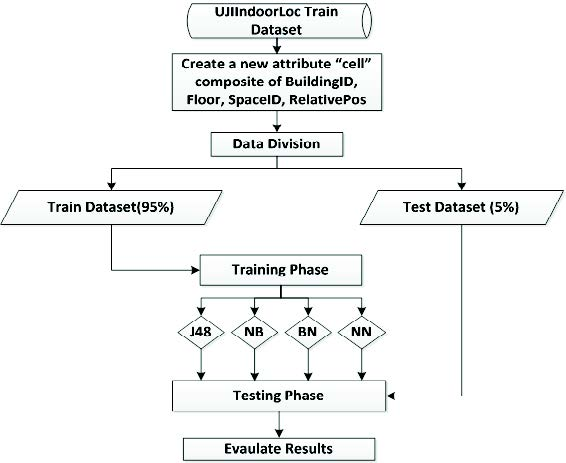
\includegraphics[scale=1]{figures/newattribute.jpg}
%		\caption{The new attribute “cell” construction phase}
%		\label{fig:newAttribute} %% NOTE: always label *after* caption!
%	\end{center}
%\end{figure}

%\todo{Compléter cette partie qui semble importante}

